\documentclass[tikz,border=5pt]{standalone}
\usepackage[T1]{fontenc}
\usepackage{amsmath,amssymb}
\usetikzlibrary{arrows.meta,positioning,calc,fit,patterns}
\begin{document}
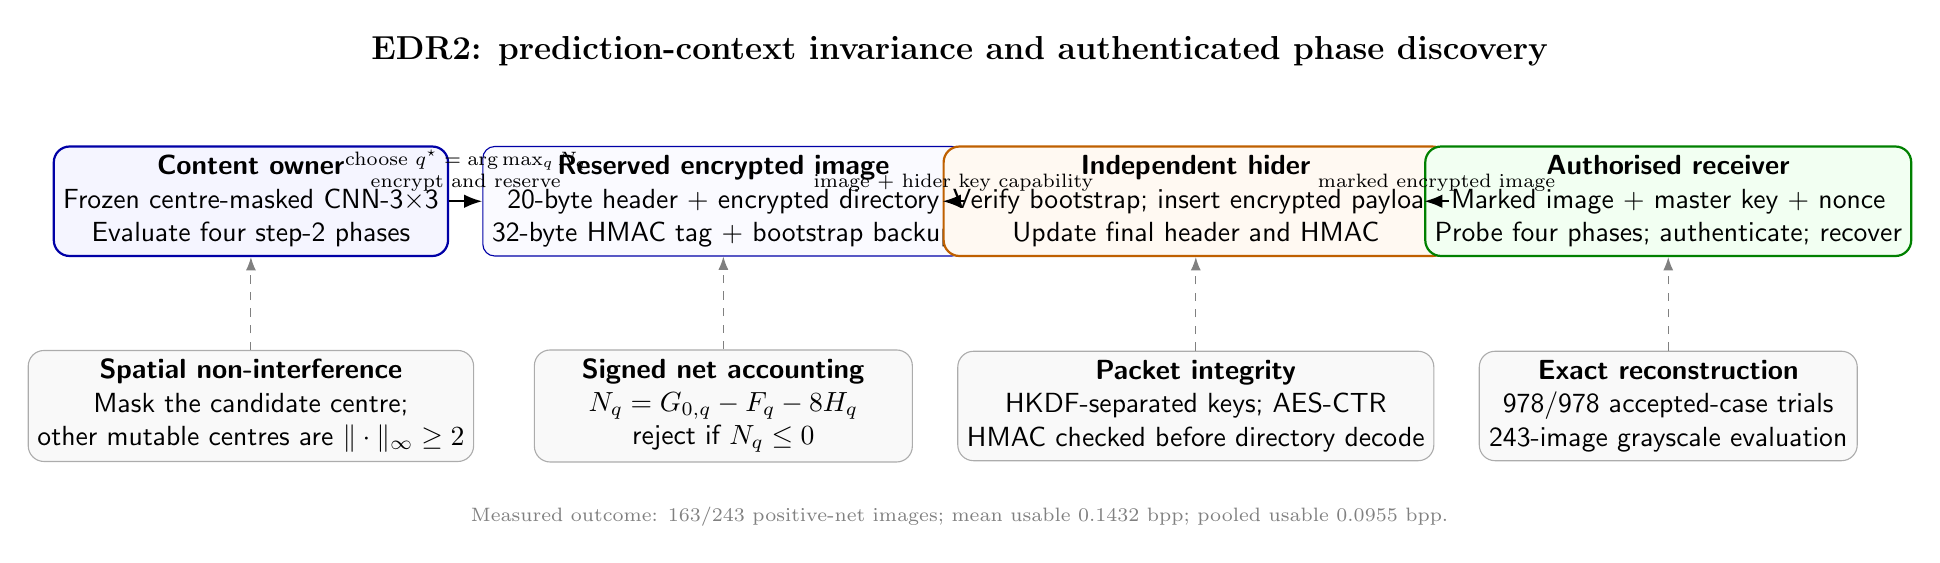
\begin{tikzpicture}[
  font=\sffamily,
  line/.style={-Latex,thick},
  owner/.style={draw=blue!65!black,fill=blue!4,rounded corners=2mm,thick,minimum width=4.8cm,minimum height=1.25cm,align=center},
  hider/.style={draw=orange!75!black,fill=orange!5,rounded corners=2mm,thick,minimum width=4.8cm,minimum height=1.05cm,align=center},
  receiver/.style={draw=green!50!black,fill=green!5,rounded corners=2mm,thick,minimum width=4.8cm,minimum height=1.25cm,align=center},
  note/.style={font=\scriptsize,align=center,text width=4.4cm}
]
\node[owner] (owner) at (0,2.5) {\textbf{Content owner}\\Frozen centre-masked CNN-3$\times$3\\Evaluate four step-2 phases};
\node[draw=blue!65!black,fill=blue!2,rounded corners=1.5mm,minimum width=4.6cm,minimum height=1.0cm,align=center] (packet) at (6,2.5) {\textbf{Reserved encrypted image}\\20-byte header + encrypted directory\\32-byte HMAC tag + bootstrap backup};
\node[hider] (hider) at (12,2.5) {\textbf{Independent hider}\\Verify bootstrap; insert encrypted payload\\Update final header and HMAC};
\node[receiver] (receiver) at (18,2.5) {\textbf{Authorised receiver}\\Marked image + master key + nonce\\Probe four phases; authenticate; recover};
\draw[line] (owner.east) -- node[above,font=\scriptsize,align=center]{choose $q^\star=\arg\max_q N_q$\\encrypt and reserve} (packet.west);
\draw[line] (packet.east) -- node[above,font=\scriptsize]{image + hider key capability} (hider.west);
\draw[line] (hider.east) -- node[above,font=\scriptsize]{marked encrypted image} (receiver.west);

\node[draw=gray!65,rounded corners=2mm,fill=gray!5,minimum width=4.8cm,minimum height=1.05cm,align=center] (geometry) at (0,-0.1) {\textbf{Spatial non-interference}\\Mask the candidate centre;\\other mutable centres are $\|\cdot\|_\infty\geq2$};
\node[draw=gray!65,rounded corners=2mm,fill=gray!5,minimum width=4.8cm,minimum height=1.05cm,align=center] (accounting) at (6,-0.1) {\textbf{Signed net accounting}\\$N_q=G_{0,q}-F_q-8H_q$\\reject if $N_q\leq0$};
\node[draw=gray!65,rounded corners=2mm,fill=gray!5,minimum width=4.8cm,minimum height=1.05cm,align=center] (auth) at (12,-0.1) {\textbf{Packet integrity}\\HKDF-separated keys; AES-CTR\\HMAC checked before directory decode};
\node[draw=gray!65,rounded corners=2mm,fill=gray!5,minimum width=4.8cm,minimum height=1.05cm,align=center] (exact) at (18,-0.1) {\textbf{Exact reconstruction}\\978/978 accepted-case trials\\243-image grayscale evaluation};
\draw[dashed,gray,-Latex] (geometry.north) -- (owner.south);
\draw[dashed,gray,-Latex] (accounting.north) -- (packet.south);
\draw[dashed,gray,-Latex] (auth.north) -- (hider.south);
\draw[dashed,gray,-Latex] (exact.north) -- (receiver.south);

\node[font=\bfseries\large] at (9,4.4) {EDR2: prediction-context invariance and authenticated phase discovery};
\node[font=\scriptsize,text=gray] at (9,-1.5) {Measured outcome: 163/243 positive-net images; mean usable 0.1432 bpp; pooled usable 0.0955 bpp.};
\end{tikzpicture}
\end{document}
